\section{Experimental Settings}

In this section, we provide a comprehensive description of the experimental configurations to ensure the reproducibility of our results. We detail the model specifications, sampling schedulers, datasets, and randomization protocols employed in our evaluations.

\subsection{Models and Schedulers}
\label{app:models_schedulers}

We conduct experiments across a diverse set of generative models. The specific sampling schedulers and hyperparameter configurations for each model are detailed below:

\begin{itemize}
    \item \textbf{Stable Diffusion v3.5}:
    We employ the Flow Matching Euler scheduler by default, while the UniPC scheduler is employed for ablation studies. For the Classifier-Free Guidance (CFG) baseline, a guidance scale of $7.0$ is applied.

    \item \textbf{Lumina-Next}:
    Inference is performed using the UniPC scheduler. The guidance scale is set to $7.0$ for the CFG baseline.

    \item \textbf{Wan2.1}:
    Similarly, this model uses the UniPC scheduler; however, the guidance scale is adjusted to $5.0$ for the CFG baseline to ensure optimal performance in video generation.

    \item \textbf{Wan2.2}: This model uses Flow Matching Euler scheduler; the guidance scale is adjusted to $5.0$ for the CFG baseline to ensure optimal performance in video generation.

    \item \textbf{Qwen-Image}: This model uses Flow Matching Euler scheduler; the guidance scale is adjusted to $4.0$ for the CFG baseline to ensure optimal performance in video generation.
    
\end{itemize}

\subsection{Datasets and Randomization}
\label{app:datasets}

To guarantee reliability and deterministic generation, we specify the datasets and seed strategies used for quantitative evaluation in the main paper:

\begin{itemize}
    
    \item \textbf{Text-to-Image Generation (\Cref{fig:txt2img_compare})}:
    Evaluations are performed on the \textbf{MS-COCO}. We construct a test set comprising the initial $500$ prompts extracted from the full dataset.
    \begin{itemize}
        \item \textbf{Randomization}: To ensure reproducibility, we adopt a deterministic strategy where the random seed for each sample is set equal to its corresponding prompt index.
    \end{itemize}

    \item \textbf{Text-to-Video Generation (\Cref{fig:txt2video_compare})}:
    Video synthesis capabilities are evaluated using \textbf{WebVid}. For this task, we randomly select a subset of $100$ samples.
    \begin{itemize}
        \item \textbf{Randomization}: The randomization protocol remains consistent with the text-to-image setting (i.e., seed equals sample index).
    \end{itemize}

    \item \textbf{Impact of Dimensionality (\Cref{tab:resolution_ir})}:
    A specific subset consisting of the first 200 prompts from \textbf{ImageReward Dataset~\citep{xu2023imagereward}} is employed for this analysis.
    \begin{itemize}
        \item \textbf{Randomization}: To maintain fixed noise initialization across experiments, the random seed is assigned to match the prompt ID of each sample.
    \end{itemize}

    \item \textbf{Orthogonality Analysis (\Cref{tab:orthogonality})}:
    We use a curated collection of 200 prompts drawn from \textbf{ImageReward Dataset}.
    \begin{itemize}
        \item \textbf{Randomization}: Stochasticity is governed by a deterministic mapping, where the seed for each generation is aligned with the prompt's index in the test suite.
    \end{itemize}

    \item \textbf{Comparison with Time-Based Schedule (\Cref{tab:time_vs_instance})}:
    Testing is conducted using the first 200 samples extracted from \textbf{ImageReward Dataset}.
    \begin{itemize}
        \item \textbf{Randomization}: We adhere to a predefined scheme in which the random seed for each instance is set equal to its sequence number in the group.
    \end{itemize}
    
\end{itemize}

\subsection{Hyper-Parameter Settings}

 For all experiments involving \mtdbk, we use the default parameters $\alpha = 8$ and $w_{\max} = 10$, which provide robust results across diverse scenarios.

In addition to \mtdbk, we detail the configurations for all baselines discussed in \Cref{subsec:txt2img_generation} as follows:

\begin{itemize}
 \item \textbf{CFG-Zero*~\citep{fan2025cfg0}:} This method is parameter-free. We strictly follow the implementation details provided in the original work.

 \item \textbf{Guidance Scheduler~\citep{xianalysis}:} We employ a cosine schedule for guidance and set the minimum guidance scale to $4.0$.

 \item \textbf{Limited Interval~\citep{kynkaanniemi2024applying}:} CFG is applied during the interval spanning $10\%$ to $90\%$ of the total sampling steps (i.e., excluding the first and last $10\%$). The guidance scale is fixed at $7.0$.
 \end{itemize}

\subsection{Prompts for Visual Examples}
\label{app:prompts}

In this subsection, we list the exact textual prompts corresponding to the visual qualitative results presented in the main paper.

\begin{description}
    \item[\Cref{fig:display} (a):]
    \textit{"Cirno, Touhou, ice fairy, light blue short hair, big blue hair ribbon, blue eyes, smug face, open mouth, confidence, blue and white dress, serrated skirt, red neckerchief, crystal wings, ice wings, floating, hands on hips, ice magic, snowflakes, frozen lake background, misty, magical atmosphere, anime style, cel shading, masterpiece, best quality, 8k, vivid colors"}

    \item[\Cref{fig:display} (b):]
    \textit{"A photograph of an astronaut riding a horse, high quality, 4k, detailed, on Moon"}

    \item[\Cref{fig:display} (c) (d):]
    \textit{"Two anthropomorphic cats in comfy boxing gear and bright gloves fight intensely on a spotlighted stage."}

    \item[\Cref{fig:resolution_comparison_4rows}:]
    \textit{"delicious plate of food"}
\end{description}


\subsection{Configurations of Exploratory Experiments}
\label{app:config_explore}

Here we specify the detailed settings for the exploratory analyses discussed in the main text.

\begin{itemize}
    \item \textbf{Collapse of Guidance Directions at Initialization (\Cref{fig:cosine_sim}):}
    These results are derived from Stable Diffusion v3.5 using a default guidance scale of $7.0$. We configure the random noise seeds and use the fixed prompts from MS-COCO.

    \item \textbf{Dynamics of the ratio during sampling (\Cref{fig:ratio_distribution_step}):}
    Ratio values are tracked using Stable Diffusion v3.5 with a guidance scale of $7.0$. The sampling process consists of 10 steps. The dataset comprises $100$ prompts from MS-COCO, following the randomization strategy defined in \Cref{subsec:txt2img_generation}.

    \item \textbf{Probability density of ImageReward scores across different ratio groups (\Cref{fig:high_ratio_vs_low_ratio}):}
    Using Stable Diffusion v3.5 (guidance scale $7.0$), we analyze the first $20$ prompts from MS-COCO. We employ a 10-step sampling procedure for each generation. For each prompt, we generate samples across $20$ distinct seeds. Ratio groups are determined via binary splitting based on the median ratio value.

    \item \textbf{Optimal Guidance Scale vs. Ratio (\Cref{fig:ratio_guidance_fit})}:
    We search for optimal guidance scales relative to observed ratio values on Stable Diffusion v3.5. A constant guidance schedule of $7.0$ serves as the baseline. The generation process uses 10 sampling steps. For the first step, we sweep the guidance scale from $1.5$ to $9.0$ in increments of $0.5$ to identify the optimal configuration, then searching for the subsequent step based on the previously optimal guidance schedule. Detailed algorithm is presented in \Cref{alg:greedy_search}. This experiment uses prompts from MS-COCO, adhering to the randomization strategy described in \Cref{subsec:txt2img_generation}.


\end{itemize}

\begin{algorithm}[t]
\caption{Greedy Search for Step-wise Optimal Guidance Scale}
\label{alg:greedy_search}
\begin{algorithmic}[1]
\REQUIRE Prompts $\mathcal{P}$ from MS-COCO, Sampling steps $T=10$, Search space $\mathcal{W} = \{1.5, 2.0, \dots, 9.0\}$, Baseline scale $w_{base} = 7.0$
\ENSURE Optimal guidance schedule $\mathbf{w}^* = (w^*_1, w^*_2, \dots, w^*_T)$
\STATE Initialize $\mathbf{w}^* = (w_{base}, w_{base}, \dots, w_{base})$ \COMMENT{Set baseline schedule}
\FOR{$t = 1$ \textbf{to} $T$}
    \STATE \COMMENT{Search for the optimal scale at current step $t$}
    \STATE $w^*_t = \arg\max_{w \in \mathcal{W}} \text{AverageMetric}\left( \text{Generate}(\mathcal{P}, \mathbf{w}_{tmp}) \right)$
    \STATE \textbf{where} $\mathbf{w}_{tmp} = (w^*_1, \dots, w^*_{t-1}, w, w_{base}, \dots, w_{base})$
    \STATE Update $\mathbf{w}^*$ with the newly found $w^*_t$
\ENDFOR
\STATE \textbf{Output:} Correlate each $w^*_t$ with the corresponding average ratio $r_t$ observed at step $t$ to analyze the trend in \Cref{fig:ratio_guidance_fit}.
\STATE \textbf{return} $\mathbf{w}^*$
\end{algorithmic}
\end{algorithm}

\section{Supplementary Results}

\subsection{Quantitative Evaluation via FID}
\label{app:exp_fid}

To rigorously assess the distributional similarity between generated images and real-world data, we evaluate \mtdbk using the Fr\'echet Inception Distance (FID) on 5,000 prompts from MS-COCO dataset. All samples are generated under the fixed seed. The results, summarized in \Cref{tab:fid_results}, demonstrate that \mtdbk significantly enhances the generative quality in low-step regimes. Specifically, at only $10$ sampling steps, \mtdbk achieves an FID of \textbf{32.05}, representing a substantial improvement over the standard CFG baseline ($63.62$). Notably, our $10$-step performance closely approaches the quality of $30$-step CFG ($24.80$), effectively bridging the gap between efficient sampling and high-fidelity generation. This confirms that \mtdbk still maintains an accurate generation trajectory even under aggressive acceleration.

\begin{table}[h]
    \centering
    \caption{\textbf{FID Results on MS-COCO.} We compare \mtdbk with standard CFG across different sampling steps. FID ($\downarrow$) measures the distributional distance to reference images (we use $50$-step CFG as reference). The results demonstrate that \mtdbk at $10$ steps significantly outperforms the $10$-step CFG baseline.}
    \label{tab:fid_results}
    \normalsize
    \begin{tabular}{lcc}
        \toprule
        Method & Sampling Steps & FID ($\downarrow$) \\
        \midrule
        CFG (Baseline) & 10 & 63.6170 \\
        CFG (Baseline) & 30 & 24.8043 \\
        \midrule
        \textbf{\mtdbk (Ours)} & \textbf{10} & \textbf{32.0545} \\
        \midrule
        CFG (Reference) & 50 & --- \\
        \bottomrule
    \end{tabular}
\end{table}



\subsection{Ablation Studies}
\label{app:exp_ablation}

In this section, we present some supplementary results of our ablation studies in \Cref{subsec:ablation}, as shown in \Cref{tab:wmax_ablation,tab:alpha_ablation,fig:unipc_ablation}.
The detailed configurations are as follows:

\begin{itemize}

    \item \textbf{Ablation studies on $w_{\max}$ (\Cref{tab:wmax_ablation}): }
    We evaluate the sensitivity of $w_{\max}$ across SD3.5 and Qwen-Image models. Experiments are conducted on the first $100$ prompts from MS-COCO, following the randomization strategy defined in \Cref{subsec:txt2img_generation}. The hyperparameter $\alpha$ is fixed at $8$, while $w_{\max}$ is varied from $6$ to $16$. Each generation is performed with $10$ sampling steps.

    \item \textbf{Ablation studies on $\alpha$ (\Cref{tab:alpha_ablation}): }
    We evaluate the sensitivity of $\alpha$ across SD3.5 and Qwen-Image models. Experiments are conducted on the first $100$ prompts from MS-COCO, following the randomization strategy defined in \Cref{subsec:txt2img_generation}. The hyperparameter $w_{\max}$ is fixed at $10$, while $\alpha$ is varied from $6$ to $16$ to observe its impact on guidance damping. Each generation is performed with $10$ sampling steps.

    \item \textbf{Ablation studies on schedulers (\Cref{fig:unipc_ablation}): }
    We evaluate the robustness of \mtdbk on the UniPC scheduler. Experiments are conducted on the first $100$ prompts from MS-COCO, following the randomization strategy outlined in \Cref{subsec:txt2img_generation}. The hyperparameter settings remain consistent with those described in \Cref{subsec:txt2img_generation}. Each generation is performed with $10$ sampling steps.

\end{itemize}



% \begin{figure*}[t]
%     \centering
%     \begin{subfigure}{0.49\textwidth}
%         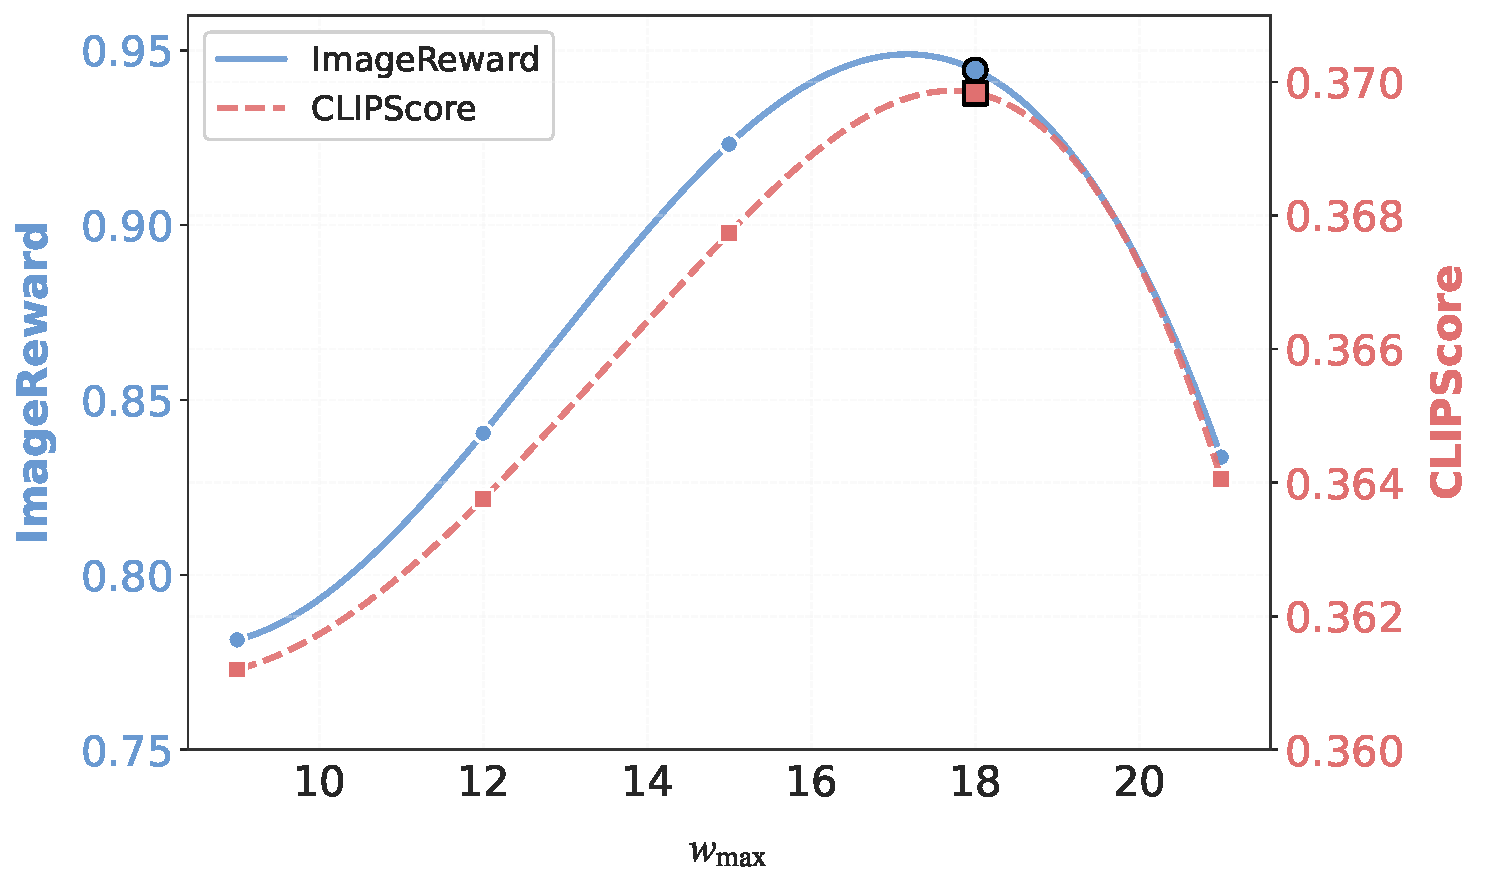
\includegraphics[width=\linewidth]{fig_tab/wmax_combined.pdf}
%         \captionsetup{justification=justified, singlelinecheck=true}
%         \caption{Ablation studies on $w_{\max}$.}
%         \label{subfig:wmax}
%     \end{subfigure}
%     \hfill 
%     \begin{subfigure}{0.49\textwidth}
%         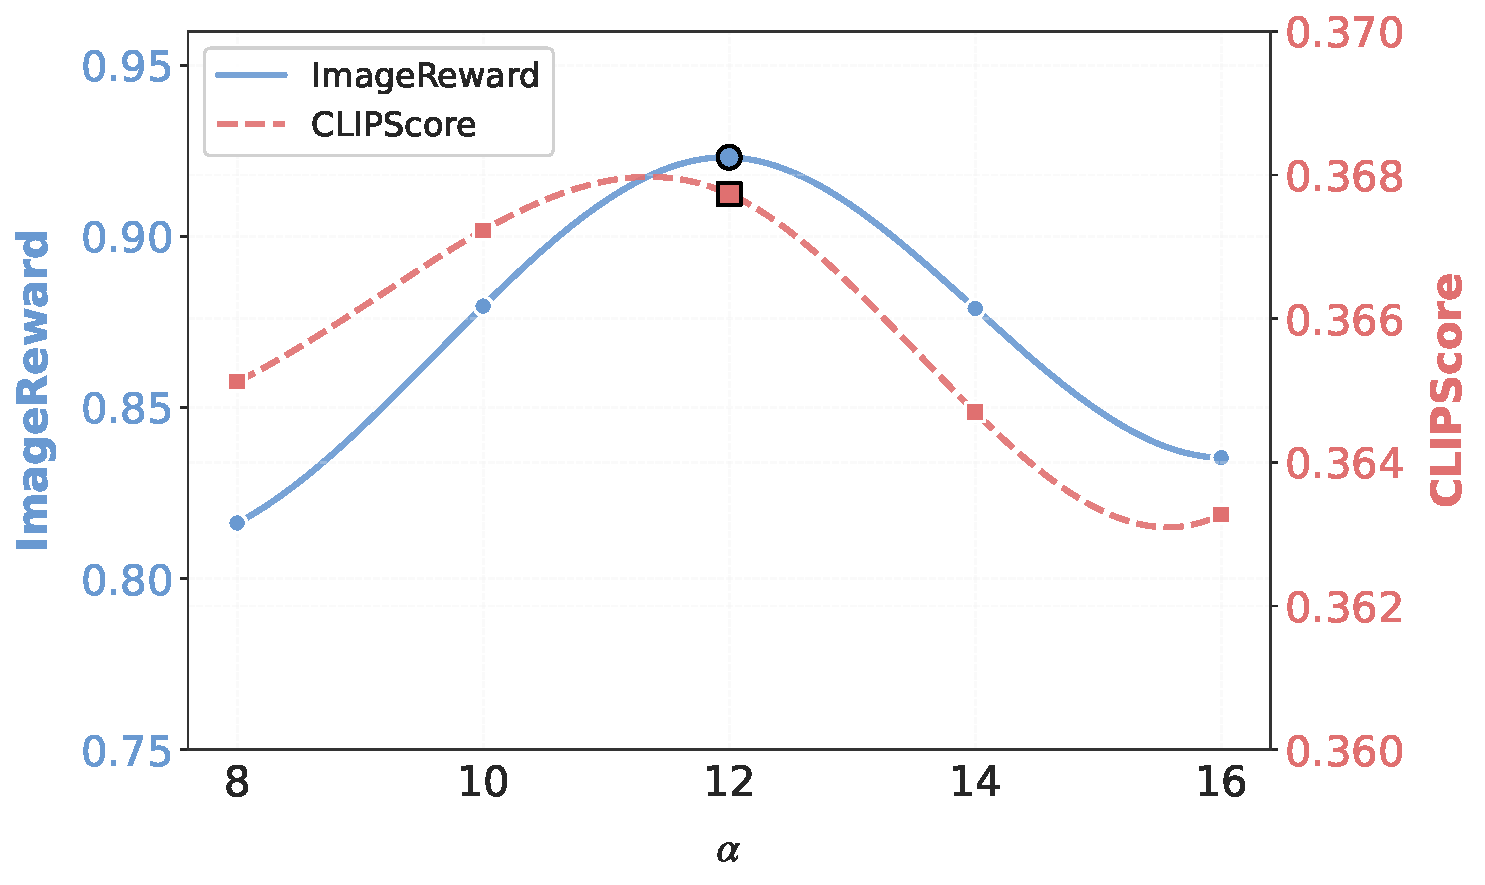
\includegraphics[width=\linewidth]{fig_tab/alpha_combined.pdf}
%         \captionsetup{justification=justified, singlelinecheck=true}
%         \caption{Ablation studies on $\alpha$.}
%         \label{subfig:alpha}
%     \end{subfigure}
%     \captionsetup{justification=justified, singlelinecheck=false}
%     \caption{Ablation studies on hyperparameters $w_{\max}$ and $\alpha$. \Cref{subfig:wmax,subfig:alpha} present the variation trends of ImageReward and CLIPScore with respect to hyperparameters and validate our optimal selection of $w_{\max}$ and $\alpha$, indicating that the generation quality of \methodabbr is largely insensitive to hyperparameter selection, with performance sustained across an extensive parameter space.}
%     \label{fig:hyper_ablation}
% \end{figure*}



% \begin{figure*}[t]
%     \centering
%     \begin{subfigure}{0.49\textwidth}
%         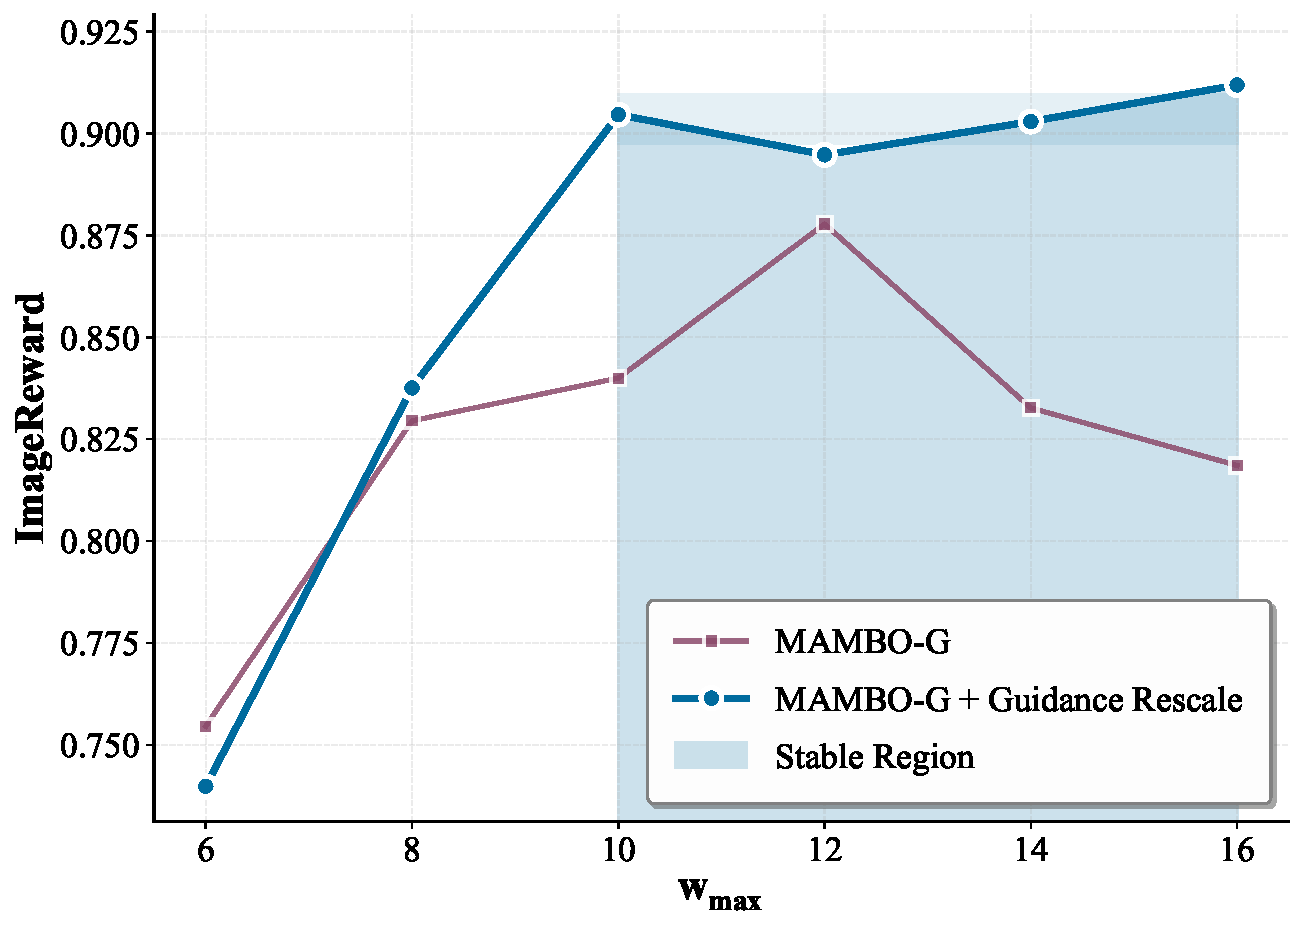
\includegraphics[width=\linewidth]{fig_tab/wmax_sensitivity_SD35.pdf}
%         \captionsetup{justification=justified, singlelinecheck=true}
%         \caption{Ablation studies of $w_{\max}$ on SD3.5.}
%         \label{subfig:wmax_sd35}
%     \end{subfigure}
%     \hfill 
%     \begin{subfigure}{0.49\textwidth}
%         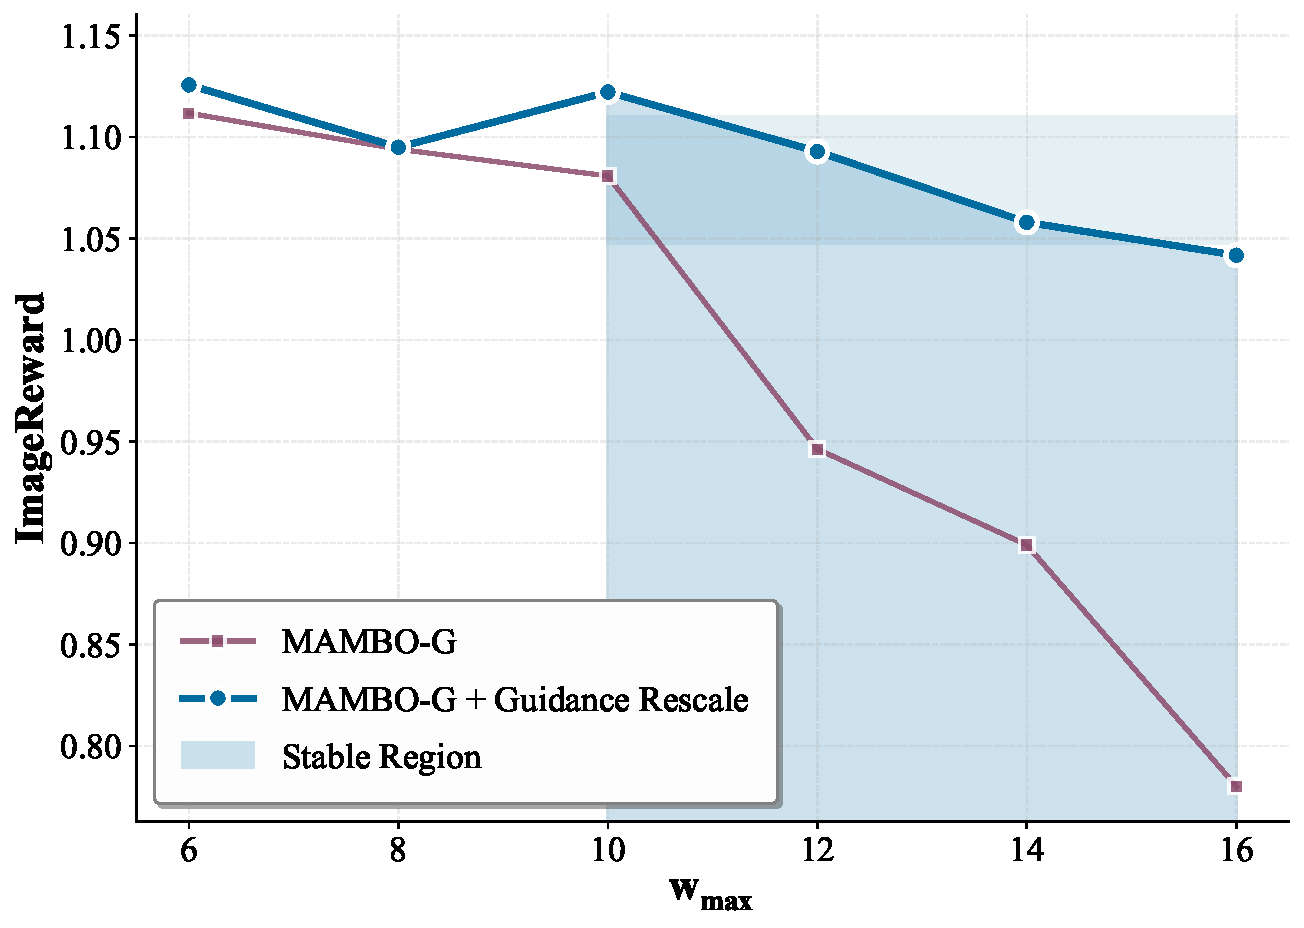
\includegraphics[width=\linewidth]{fig_tab/wmax_sensitivity_Qwen.pdf}
%         \captionsetup{justification=justified, singlelinecheck=true}
%         \caption{Ablation studies of $w_{\max}$ on Qwen-Image.}
%         \label{subfig:wmax_qwen}
%     \end{subfigure}
%     \begin{subfigure}{0.49\textwidth}
%         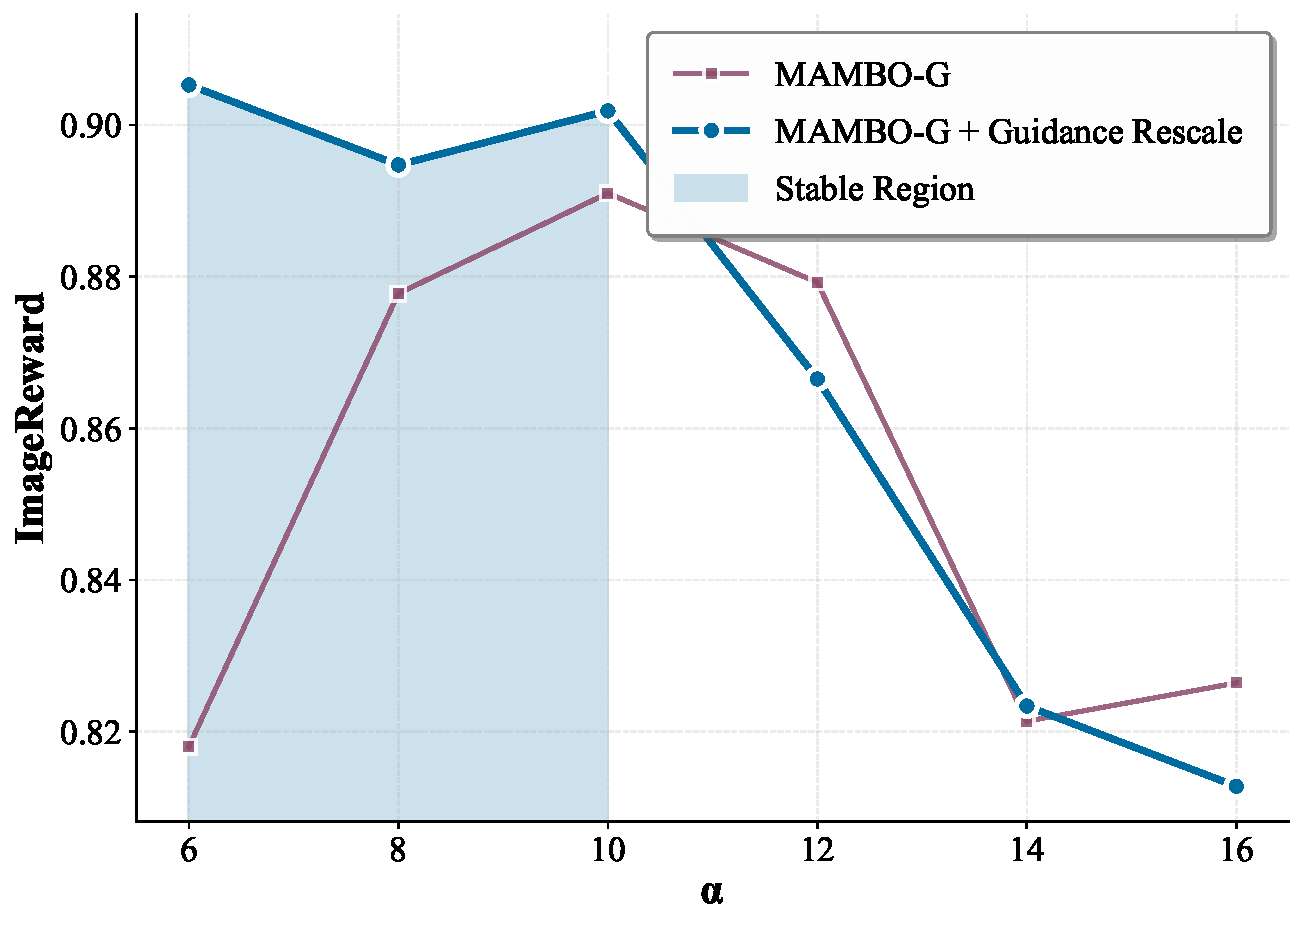
\includegraphics[width=\linewidth]{fig_tab/alpha_sensitivity_SD3.5_wmax12.pdf}
%         \captionsetup{justification=justified, singlelinecheck=true}
%         \caption{Ablation studies of $\alpha$ on SD3.5.}
%         \label{subfig:alpha_sd35}
%     \end{subfigure}
%     \hfill 
%     \begin{subfigure}{0.49\textwidth}
%         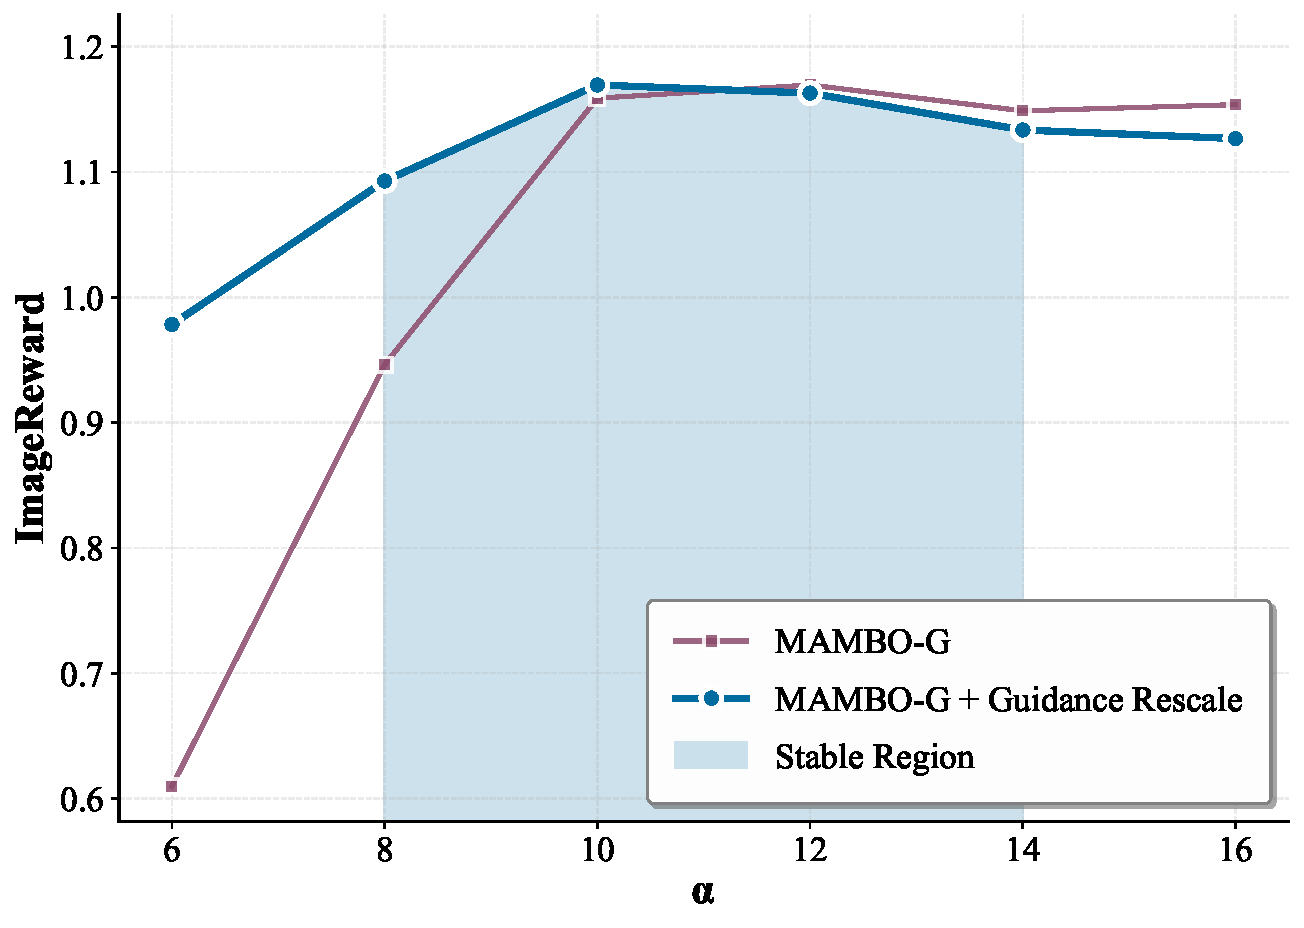
\includegraphics[width=\linewidth]{fig_tab/alpha_sensitivity_Qwen_wmax12.pdf}
%         \captionsetup{justification=justified, singlelinecheck=true}
%         \caption{Ablation studies of $\alpha$ on Qwen-Image.}
%         \label{subfig:alpha_qwen}
%     \end{subfigure}
%     \captionsetup{justification=justified, singlelinecheck=false}
%     \caption{Ablation studies on hyperparameters $w_{\max}$ and $\alpha$ across different models. \Cref{subfig:wmax_sd35,subfig:wmax_qwen,subfig:alpha_sd35,subfig:alpha_qwen} demonstrate the remarkable stability of \mtdbk when combined with Guidance Rescale, maintaining consistently high performance across an extensive parameter space with insensitivity to hyperparameter selection.}
%     \label{fig:hyper_ablation}
% \end{figure*}

\begin{table}[htbp]
\centering
\caption{Ablation studies on hyperparameter $w_{\max}$ (with fixed $\alpha=8$) across different models. The scores represent ImageReward, with the best performance in each row highlighted in \textbf{bold}.}
\label{tab:wmax_ablation}
\begin{tabular}{llcccccc}
\toprule
\multirow{2}{*}{\textbf{Model}} & \multirow{2}{*}{\textbf{Method}} & \multicolumn{6}{c}{\textbf{$w_{\max}$}} \\
\cmidrule(lr){3-8}
 & & \textbf{6} & \textbf{8} & \textbf{10} & \textbf{12} & \textbf{14} & \textbf{16} \\ 
\midrule
\multirow{2}{*}{SD3.5} & \mtdbk & 0.755 & 0.830 & 0.840 & \textbf{0.878} & 0.833 & 0.819 \\
 & \mtdbk + Rescale & 0.740 & 0.838 & 0.905 & 0.895 & 0.903 & \textbf{0.912} \\ 
\midrule
\multirow{2}{*}{Qwen-Image} & \mtdbk & \textbf{1.112} & 1.094 & 1.081 & 0.946 & 0.899 & 0.780 \\
 & \mtdbk + Rescale & \textbf{1.126} & 1.095 & 1.122 & 1.093 & 1.058 & 1.042 \\ 
\bottomrule
\end{tabular}
\end{table}

\begin{table}[htbp]
\centering
\caption{Ablation studies on hyperparameter $\alpha$ (with fixed $w_{\max}=10$) across different models. The scores represent ImageReward, with the best performance in each row highlighted in \textbf{bold}.}
\label{tab:alpha_ablation}
\begin{tabular}{llcccccc}
\toprule
\multirow{2}{*}{\textbf{Model}} & \multirow{2}{*}{\textbf{Method}} & \multicolumn{6}{c}{\textbf{$\alpha$}} \\
\cmidrule(lr){3-8}
 & & \textbf{6} & \textbf{8} & \textbf{10} & \textbf{12} & \textbf{14} & \textbf{16} \\ 
\midrule
\multirow{2}{*}{SD3.5} & \mtdbk & 0.827 & 0.840 & \textbf{0.857} & 0.817 & 0.785 & 0.774 \\
 & \mtdbk + Rescale & 0.875 & \textbf{0.905} & 0.867 & 0.818 & 0.808 & 0.768 \\ 
\midrule
\multirow{2}{*}{Qwen-Image} & \mtdbk & 0.830 & 1.081 & 1.156 & \textbf{1.161} & 1.132 & 1.122 \\
 & \mtdbk + Rescale & 1.010 & 1.122 & \textbf{1.155} & 1.142 & 1.136 & 1.130 \\ 
\bottomrule
\end{tabular}
\end{table}

\begin{figure}[h]
    \centering
    \begin{subfigure}{0.49\textwidth}
        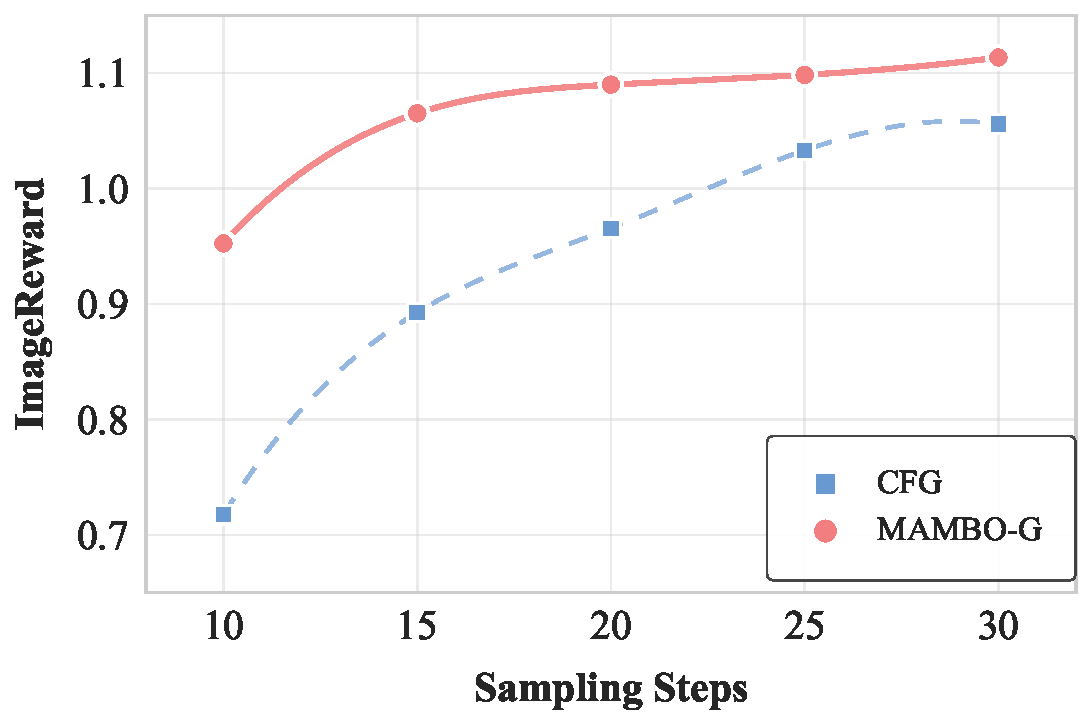
\includegraphics[width=\linewidth]{fig_tab/SD35_UniPC_ImageReward_comparison.pdf}
        \captionsetup{justification=justified, singlelinecheck=true}
        \caption{SD3.5 UniPC, ImageReward.}
        \label{fig:sub1_1}
    \end{subfigure}
    \hfill
    \begin{subfigure}{0.49\textwidth}
        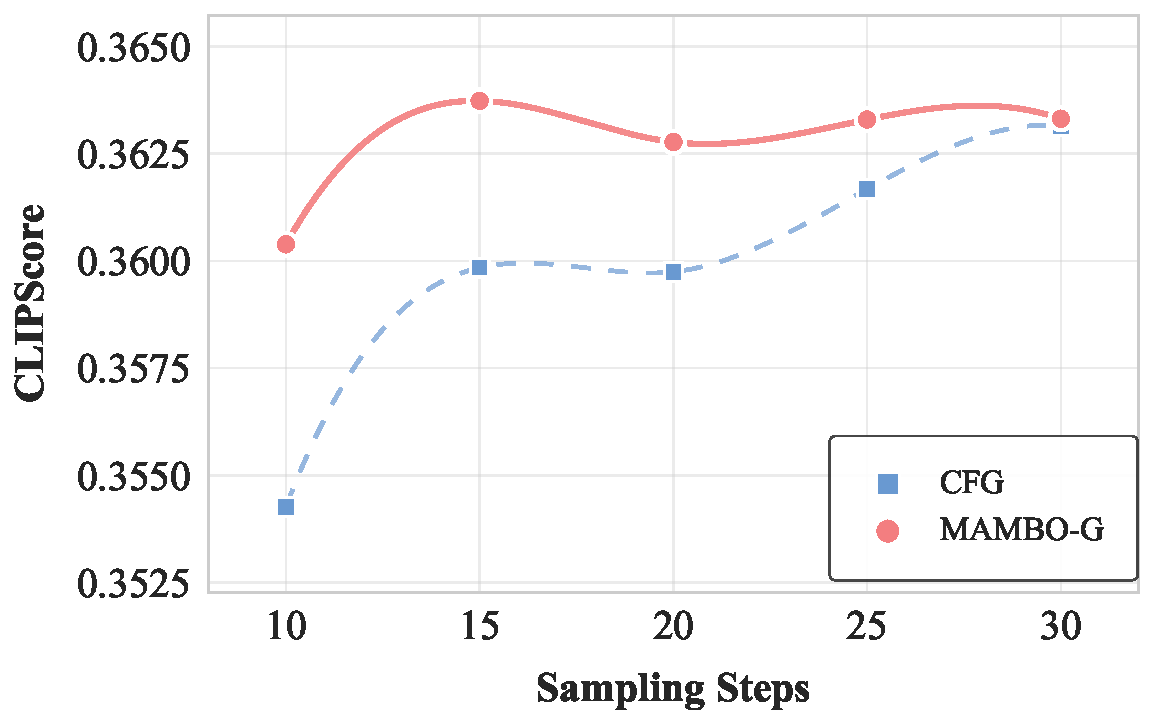
\includegraphics[width=\linewidth]{fig_tab/SD35_UniPC_CLIPScore_comparison.pdf}
        \captionsetup{justification=justified, singlelinecheck=true}
        \caption{SD3.5 UniPC, CLIPScore.}
        \label{fig:sub1_2}
    \end{subfigure}
    \captionsetup{justification=justified, singlelinecheck=false}
    \caption{Ablation studies of schedulers on UniPC. The comparative results present the consistent superiority of \mtdbk over CFG across different schedulers, further validating the wide-ranging adaptability of our method.}
    \label{fig:unipc_ablation}
\end{figure}